\section{Introduction}

These days, people are crazy about exploring habitable planets and extraterrestrial intelligence. Meanwhile, UFO events have been happening around us for decades, and people tell their UFO encounters in thousands of ways. Predicting any aspects about UFO is intriguing since these tiny fickle light dots leave us little trace behind.

In this project, we try to investigate this topic in three steps. First, we figure out correlations between UFO sightings and data from other sources, such as geometry, weather, population and territory area. Second, based on statistic analysis and machine learning techniques, we develop models to detect fake UFO reports. Finally, we build up a web application to visualize our analysis results and to provide users a way to interact with our project, such as enabling them to report their own sightings and get access to fake detection result.

The whole data pipeline of our project is illustrated in figure \ref{architecture}. For the rest part of our project report,  we will first discuss about data processing in section \ref{data}, and statistic analysis on UFO data in section \ref{statistic}. Machine learning methods will be indicated in section \ref{ml}. As for web application,  we will demonstrate the data pipeline and how our system works in section \ref{methodology}. In section \ref{challenge}, we will discuss the challenges we met during working on this project. Finally, in section \ref{conclusion}, we will claim the conclusions as well as future work. In section \ref{ack}, we give our profound acknowledgement to all people who help us with the project.

\begin{figure}[H]
    \centering
    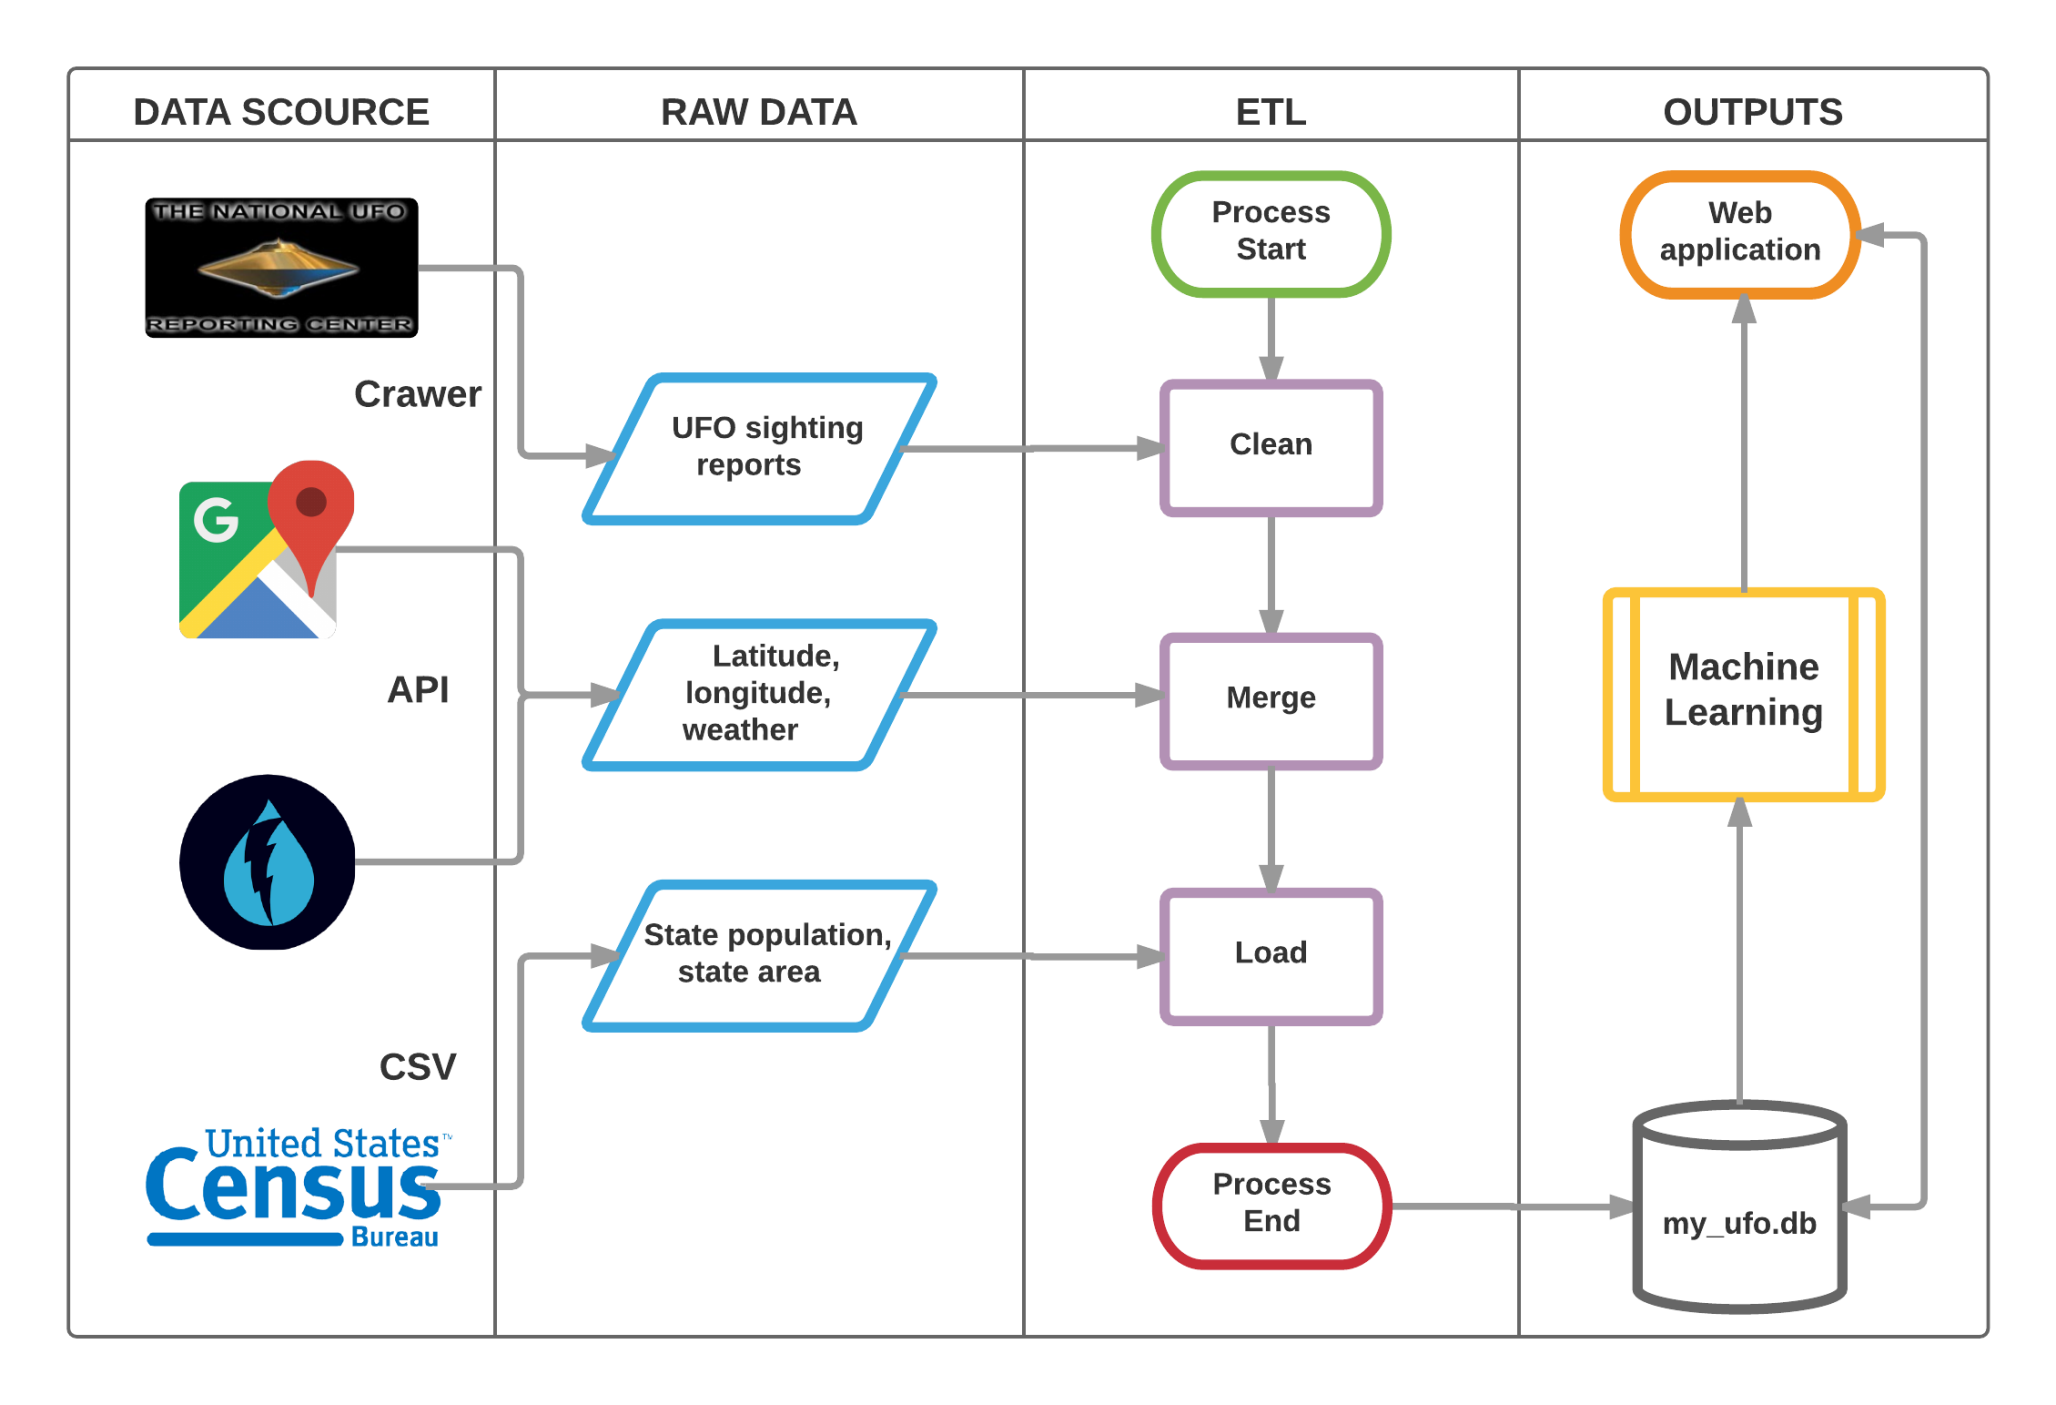
\includegraphics[width=14cm]{figure/architecture.png}
    \caption{data pipeline architecture}
    \label{architecture}
\end{figure}